\documentclass[11pt]{article}

\usepackage{custom}

\title{605.744: Information Retrieval \\ Programming Assignment \#5: Near Duplicate Detection}
\author{Sabbir Ahmed}
\date{\today}

\begin{document}
\maketitle
\tableofcontents
\clearpage
\newpage

\section{Introduction}
This paper describes detecting near-duplications (plagiarism) within documents in datasets of various sample sizes.

\section{Technical Background}
All of the source code is in Python 3.10. The program is split into several modules and follows an object oriented structure.

% .
% ├── ir/
% │   ├── __init__.py
% │   ├── files.py
% │   ├── minhash.py
% │   └── text.py
% ├── models/
% ├── outputs/
% └── run.py

\begin{figure}[!ht]
  \centering
  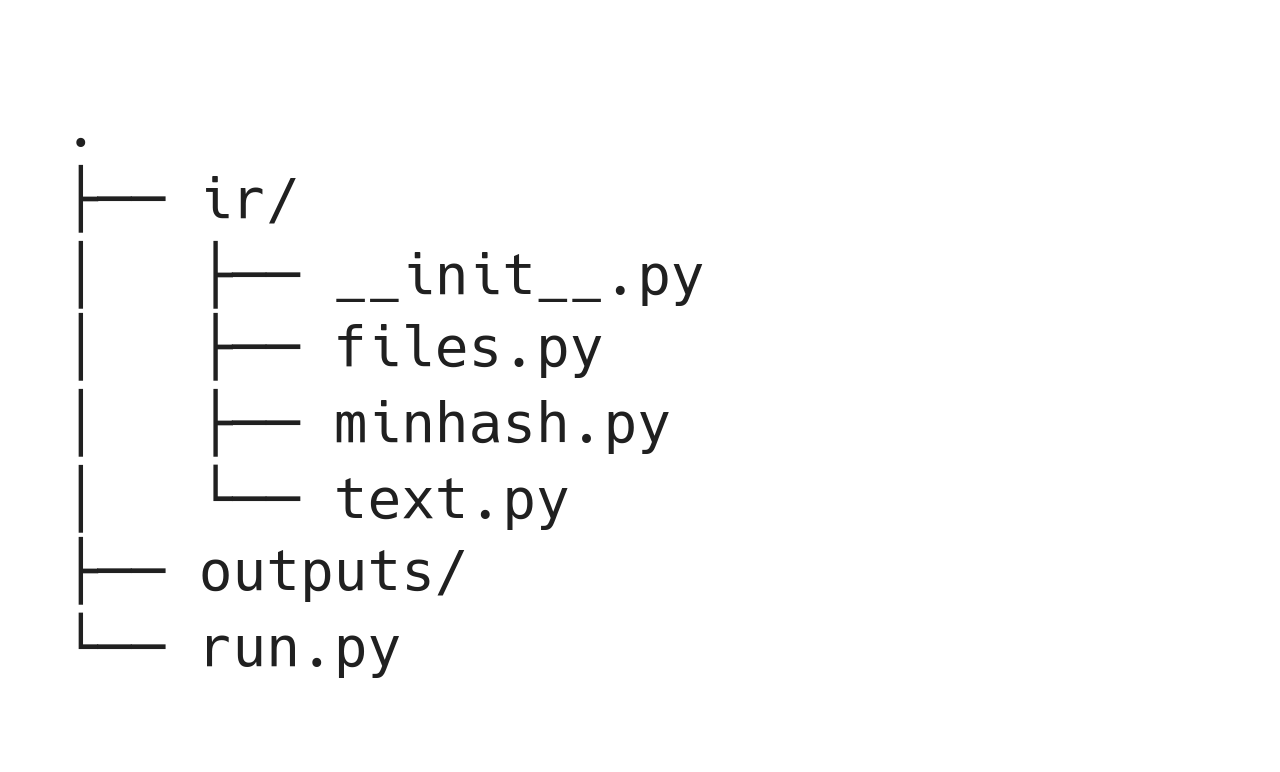
\includegraphics[trim={0 3cm 15cm 3cm},clip,scale=0.3]{statics/dirtree.png}
  \caption{Directory Hierarchy of Assignment 5}
\end{figure}

The source code for all of the files are attached in Appendix \ref{appendix:src}.

The total number of non-empty lines of code for the program totals to under 285.

\begin{figure}[!ht]
  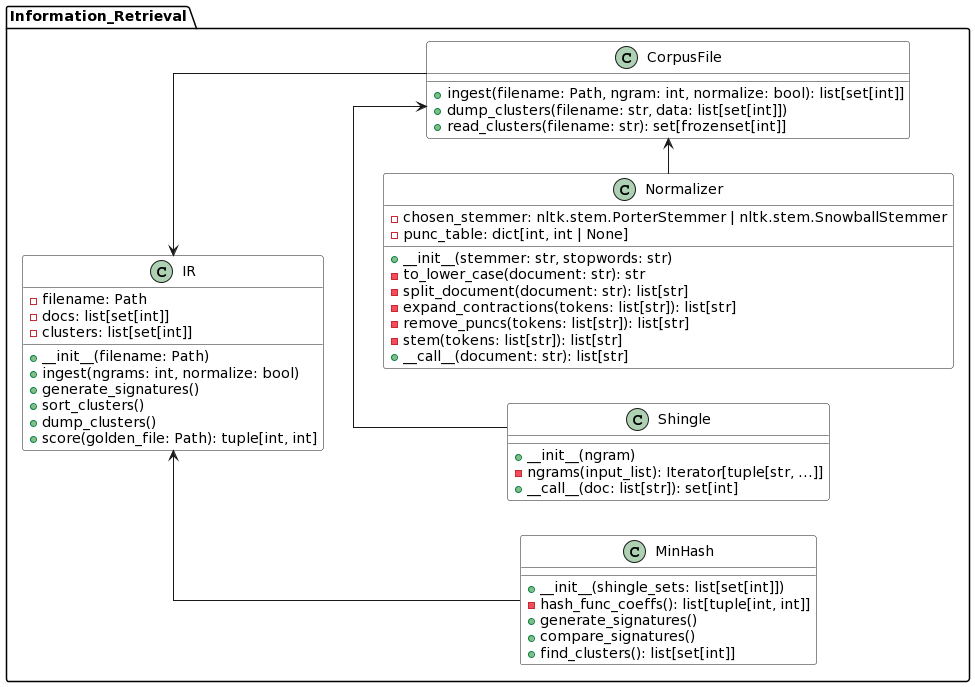
\includegraphics[scale=0.45]{statics/uml.png}
  \centering
  \caption{UML of Information Retrieval}
\end{figure}

\subsection{Classes}
Some classes from Assignment 3 were used in this project:
\begin{itemize}
  \item the driver script \texttt{run.py} was modified with the relevant flags
  \item the \texttt{files.CorpusFile} class was modified to process TSV files and read and write clusters to disk
  \item the \texttt{text.Normalizer} class was used to normalize documents into lists of stemmed words
\end{itemize}

\subsection{\texttt{text.Shingle}}
The \texttt{text.Shingle} class was added to create shingles of n-grams of the documents. Each of the n-grams were stored as unique integers, $-2^{64}-1 \le x \le 2^{64}-1$, generated by Python's built-in \texttt{hash()} function.

\subsection{\texttt{minhash.MinHash}}
The \texttt{minhash.MinHash} class was added to generate the signatures from the shingles and determine clusters of near-duplicate documents. The algorithm for generating and comparing the min-hash values was based on the column-row permutations described in \textit{Mining Massive Datasets} \cite{leskovec_rajaraman_ullman_2022}. A min hash signature, $\Phi_s$, is generated by the precomputed hash functions, The hash functions $\{h_1(x),h_2(x),...,h_{200}(x)\}$ are precomputed, of the form $h(x)=(a \times x + b) \ mod \ p$, where $p$ is prime and the random coefficients, $\{a,b \in \mathbb{N}: 0 \le a,b \le 2^{32}-1\}$. For this function, $p$ is chosen to be $4,294,967,295$, the first prime number larger than $2^{32}-1$.

The min-hashing method was derived from the pseudocode detailed in the \textit{MIN-HASHING AND LOCALITY SENSITIVE HASHING} slides \cite{kollios}.

The signatures are stored in a $N \times N$ matrix. The occurrences of matching signatures are tallied up and used to determine near-duplication if they exceed the threshold value.

\subsection{External Libraries}
The following external libraries were used to implement portions of the assignment:
\begin{itemize}
  \item Natural Language Toolkit (NLTK) \cite{bird2009natural}, for its Snowball stemmer
  \item NetworkX \cite{SciPyProceedings_11}, for its UnionFind data structure
\end{itemize}

\section{Scoring}
The golden file provided for the \texttt{twok} dataset was used to gauge the performance of the assignment. The evaluations were computed using the cardinalities of the set-difference sets $(|G-O|,|O-G|)$, where $G$ represents the clusters of the golden file and $O$ represents the generated clusters. This ad-hoc metric shows how many generated clusters were mismatched from their expected grouping.

Various combinations of n-grams and normalization were used to determine the best approach to yield the best performance. Table \ref{table:scores} shows the scores generated.

\begin{simptable}
  {Cardinalities of set-difference sets with various n-grams and normalization parameters}
  {scores}
  {| c | c | c | c |}
  \textbf{N-Gram} & \textbf{Normalized} & \textbf{$|G-O|$} & \textbf{$|O-G|$}
  \\ \hline
  \textbf{6} & True & 10 & 12
  \\ \hline
  \textbf{6} & False & 10 & 12
  \\ \hline
  \textbf{5} & True & 3 & 6
  \\ \hline
  \textbf{5} & False & 4 & 9
  \\ \hline
  \textbf{4} & True & 3 & 6
  \\ \hline
  \textbf{4} & False & 3 & 6
  \\ \hline
  \textbf{3} & True & 2 & 4
  \\ \hline
  \textbf{3} & False & 2 & 4
  \\ \hline
  \textbf{2} & True & 1 & 2
  \\ \hline
  \textbf{2} & False & 3 & 2
  \\ \hline
  \textbf{1} & True & 2 & 1
  \\ \hline
  \textbf{1} & False & 2 & 2
  \\ \hline
\end{simptable}

The best parameters were determined to be 2-grams with text normalization. These parameters were used to generate the clusters for the 30, 100, 300, 1,000, 3,000, 10,000 and 30,000 document datasets.

\section{Experiment}

The 30, 100, 300, 1,000, 3,000, and 10,000 document datasets were processed on a 64-bit Linux-based virtual machine with 4-cores and 4 GB of RAM. The 30,000 document dataset was processed on a 64-bit Windows machine with 32-cores and 32 GB of RAM. The total execution times are listed on Table \ref{table:times}.

The program could not process the 100,000 document dataset due to memory constraints, even on the Windows machine. The bottleneck can be pinpointed to the increasing memory requirements of assigning non-zero integers to the $100,000 \times 100,000$ signature count matrix.

\begin{simptable}
  {Total execution times of processing the datasets}
  {times}
  {| r | r |}
  \textbf{Dataset} & \textbf{Time (s)}
  \\ \hline
  30 & 0.38
  \\ \hline
  100 & 4.82
  \\ \hline
  300 & 11.14
  \\ \hline
  1,000 & 42.22
  \\ \hline
  3,000 & 170.38
  \\ \hline
  10,000 & 1280.42
  \\ \hline
  30,000 & 6132.88
  \\ \hline
\end{simptable}

\newpage
\addcontentsline{toc}{section}{References}
\bibliographystyle{ieeetr}
\bibliography{refs}

\appendix
\addcontentsline{toc}{section}{Appendix}

\section{Source Code} \label{appendix:src}

\inputpython{../ir/\_\_init\_\_.py}{ir/\_\_init\_\_.py}
\inputpython{../ir/files.py}{ir/files.py}
\inputpython{../ir/minhash.py}{ir/minhash.py}
\inputpython{../ir/text.py}{ir/text.py}

\inputpython{../run.py}{run.py}

\end{document}
